\documentclass[aspectratio=169,11pt]{beamer}

% Présentation doctorale construite à partir du mémoire, sans modifier les sources
% du mémoire, de l'article, ni l'ancien support de présentation.
\usepackage[utf8]{inputenc}
\usepackage[T1]{fontenc}
\usepackage[round,authoryear]{natbib}
\usepackage[french,shorthands=off]{babel}
\usepackage{lmodern}
\usepackage{microtype}
\usepackage{graphicx}
\usepackage{booktabs}
\usepackage{tabularx}
\usepackage{array}
\usepackage{amsmath,amssymb}
\usepackage{tikz}
\usetikzlibrary{arrows.meta,positioning,calc,shapes.geometric}

\definecolor{KmerNavy}{HTML}{0B2A67}
\definecolor{KmerBlue}{HTML}{174A9C}
\definecolor{KmerMagenta}{HTML}{A40E61}
\definecolor{KmerTeal}{HTML}{008C95}
\definecolor{KmerGreen}{HTML}{15905B}
\definecolor{KmerGold}{HTML}{B88A00}
\definecolor{KmerPurple}{HTML}{6D2B83}
\definecolor{KmerLilac}{HTML}{A87AA4}
\definecolor{KmerRed}{HTML}{B94343}
\definecolor{KmerGray}{HTML}{F2F4F7}
\definecolor{KmerDarkGray}{HTML}{344054}

\setbeamertemplate{navigation symbols}{}
\setbeamercolor{normal text}{fg=black,bg=white}
\setbeamercolor{structure}{fg=KmerNavy}
\setbeamerfont{frametitle}{series=\bfseries,size=\large}
\setbeamerfont{title}{series=\bfseries,size=\LARGE}
\setbeamerfont{subtitle}{size=\large}
\setbeamersize{text margin left=0.72cm,text margin right=0.72cm}

\newcommand{\kmerlogo}{
\includegraphics[height=0.76cm]{figures/kmerai.png}}
\newcommand{\metric}[1]{\textcolor{KmerNavy}{\bfseries #1}}
\newcommand{\sourceNote}[1]{%
  \vfill\par\tiny\color{KmerDarkGray}\textit{Source : #1}\par
}
\newcommand{\pill}[2]{%
  \tikz[baseline=(n.base)]\node[rounded corners=2pt,fill=#1!12,draw=#1!55,
  inner xsep=5pt,inner ysep=2.5pt,text=#1,font=\bfseries\scriptsize] (n) {#2};%
}

\newcommand{\segmentcolor}[1]{%
  \ifnum\value{section}=#1 KmerNavy\else KmerLilac\fi
}

\setbeamertemplate{frametitle}{%
  \nointerlineskip
  \begin{beamercolorbox}[wd=\paperwidth,ht=1.13cm,dp=0.12cm]{frametitle}
    \hbox to \paperwidth{%
      \hspace*{0.22cm}\raisebox{-0.18cm}{\kmerlogo}%
      \hspace*{0.30cm}%
      \parbox[c][0.84cm][c]{0.78\paperwidth}{\raggedright\usebeamerfont{frametitle}\insertframetitle}%
      \hfill\raisebox{-0.18cm}{\kmerlogo}\hspace*{0.22cm}%
    }
  \end{beamercolorbox}%
  \vspace{-0.08cm}
  \hspace*{1.32cm}\color{KmerMagenta}\rule{0.75\paperwidth}{1.1pt}
  \vspace{0.08cm}
}

\setbeamertemplate{footline}{%
  \leavevmode
  \hbox{%
    \begin{beamercolorbox}[wd=.315\paperwidth,ht=0.42cm,dp=0.15cm,center]{author in head/foot}%
      \colorbox{\segmentcolor{1}}{\parbox[c][0.42cm][c]{\dimexpr.315\paperwidth-2\fboxsep\relax}{\centering\color{white}\bfseries\scriptsize 1. PREUVES DU MÉMOIRE}}
    \end{beamercolorbox}%
    \begin{beamercolorbox}[wd=.315\paperwidth,ht=0.42cm,dp=0.15cm,center]{title in head/foot}%
      \colorbox{\segmentcolor{2}}{\parbox[c][0.42cm][c]{\dimexpr.315\paperwidth-2\fboxsep\relax}{\centering\color{white}\bfseries\scriptsize 2. PROGRAMME DOCTORAL}}
    \end{beamercolorbox}%
    \begin{beamercolorbox}[wd=.315\paperwidth,ht=0.42cm,dp=0.15cm,center]{date in head/foot}%
      \colorbox{\segmentcolor{3}}{\parbox[c][0.42cm][c]{\dimexpr.315\paperwidth-2\fboxsep\relax}{\centering\color{white}\bfseries\scriptsize 3. PARTENARIAT SCIENTIFIQUE}}
    \end{beamercolorbox}%
    \begin{beamercolorbox}[wd=.055\paperwidth,ht=0.42cm,dp=0.15cm,center]{page number in head/foot}%
      \colorbox{KmerNavy}{\parbox[c][0.42cm][c]{\dimexpr.055\paperwidth-2\fboxsep\relax}{\centering\color{white}\bfseries\scriptsize\insertframenumber}}
    \end{beamercolorbox}%
  }
}

\setbeamercolor{block title}{fg=white,bg=KmerNavy}
\setbeamercolor{block body}{fg=black,bg=KmerGray}
\setbeamercolor{alerted text}{fg=KmerMagenta}
\setbeamertemplate{itemize item}{\color{KmerMagenta}$\blacktriangleright$}
\setbeamertemplate{itemize subitem}{\color{KmerTeal}$\bullet$}

\title{IA hybride, explicable et responsable\\pour l'appariement emploi--compétences}
\subtitle{Du mémoire d'ingénieur à un programme doctoral falsifiable et utile}
\author{Irch Defluviaire NGOULOU NGOUBILI}
\institute{Ingénieur Statisticien Économiste — Data Science \& Marketing}
\date{Entretien en vue d'un projet doctoral — Août 2026}

\begin{document}

% -----------------------------------------------------------------------------
% PAGE DE TITRE — identité graphique conservée : blanc, bleu, filet magenta,
% logos KmerAI et navigation inférieure tricolore.
% -----------------------------------------------------------------------------
\begin{frame}[plain]
  \begin{tikzpicture}[remember picture,overlay]
    \fill[KmerNavy] (current page.north west) rectangle
      ([yshift=-1.20cm]current page.north east);
    \fill[KmerMagenta] ([yshift=-1.20cm]current page.north west) rectangle
      ([yshift=-1.27cm]current page.north east);
    \node[anchor=north west] at ([xshift=0.28cm,yshift=-0.12cm]current page.north west)
      {
\includegraphics[height=0.88cm]{figures/kmerai.png}};
    \node[anchor=north east] at ([xshift=-0.28cm,yshift=-0.12cm]current page.north east)
      {
\includegraphics[height=0.88cm]{figures/kmerai.png}};
    \fill[KmerLilac] (current page.south west) rectangle
      ([xshift=.315\paperwidth,yshift=.55cm]current page.south west);
    \fill[KmerGold] ([xshift=.315\paperwidth]current page.south west) rectangle
      ([xshift=.630\paperwidth,yshift=.55cm]current page.south west);
    \fill[KmerNavy] ([xshift=.630\paperwidth]current page.south west) rectangle
      ([yshift=.55cm]current page.south east);
  \end{tikzpicture}
  \vspace{0.72cm}
  \begin{center}
    {\color{KmerNavy}\bfseries\fontsize{22}{25}\selectfont
      IA hybride, explicable et responsable\par
      pour l'appariement emploi--compétences}

    \vspace{0.24cm}
    {\color{KmerMagenta}\rule{0.78\linewidth}{1.3pt}}

    \vspace{0.28cm}
    {\Large\bfseries Du mémoire d'ingénieur à un programme doctoral}

    \vspace{0.20cm}
    {\large\color{KmerDarkGray}
      Transformer un prototype prometteur en connaissance scientifique robuste,
      reproductible et évaluée par ses utilisateurs}

    \vspace{0.36cm}
    {\large\bfseries Irch Defluviaire NGOULOU NGOUBILI}\par
    \small Ingénieur Statisticien Économiste — Data Science \& Marketing\par
    \vspace{0.12cm}
    \pill{KmerTeal}{RECHERCHE D'ENCADREMENT DOCTORAL}

    \vspace{0.18cm}
    {\small Août 2026}
  \end{center}
\end{frame}

\section{Preuves du mémoire}

\begin{frame}{La thèse commence là où le mémoire s'arrête}
  \begin{columns}[T,onlytextwidth]
    \column{0.31\textwidth}
      \begin{block}{Le problème}
        Offres, profils et compétences utilisent des vocabulaires hétérogènes.
        Une similarité textuelle élevée ne garantit ni la compatibilité ni
        l'explicabilité.
      \end{block}
    \column{0.31\textwidth}
      \begin{block}{Le prototype}
        Une chaîne opérationnelle combine recherche sémantique, graphe de
        connaissances, \textit{skill gap} et génération contrôlée.
      \end{block}
    \column{0.31\textwidth}
      \begin{block}{Le verrou scientifique}
        Les gains observés reposent encore sur un proxy interne : la validité
        métier, la robustesse et l'effet sur la décision restent à établir.
      \end{block}
  \end{columns}
  \vspace{0.28cm}
  \begin{center}
    \pill{KmerMagenta}{MA PROPOSITION}\quad
    \textbf{faire de ces limites le cœur d'un programme doctoral testable.}
  \end{center}
  \sourceNote{Mémoire, introduction générale et conclusion ; cadre d'aide à la décision inspiré de \citep{mortensen1994job,pissarides2000equilibrium}.}
\end{frame}

\begin{frame}{Le problème scientifique : trois erreurs à éviter}
  \begin{center}
  \begin{tikzpicture}[node distance=0.58cm, every node/.style={font=\small}]
    \node[rounded corners,draw=KmerBlue,very thick,fill=KmerBlue!8,
      minimum width=3.6cm,minimum height=1.20cm,align=center] (v)
      {\textbf{Vecteur seul}\\proche sémantiquement\\$\neq$ compatible};
    \node[rounded corners,draw=KmerGreen,very thick,fill=KmerGreen!8,
      minimum width=3.6cm,minimum height=1.20cm,align=center,right=of v] (g)
      {\textbf{Graphe seul}\\relations explicites\\$\neq$ rappel suffisant};
    \node[rounded corners,draw=KmerMagenta,very thick,fill=KmerMagenta!8,
      minimum width=3.6cm,minimum height=1.20cm,align=center,right=of g] (l)
      {\textbf{LLM seul}\\explication plausible\\$\neq$ preuve};
    \node[rounded corners,draw=KmerNavy,fill=KmerNavy,text=white,
      minimum width=11.3cm,minimum height=0.92cm,align=center,
      below=0.62cm of g] (h)
      {\bfseries Récupérer $\rightarrow$ vérifier $\rightarrow$ expliquer avec preuves
       $\rightarrow$ décision humaine};
    \draw[-{Stealth},thick,KmerNavy] (v.south) -- (h.north west);
    \draw[-{Stealth},thick,KmerNavy] (g.south) -- (h.north);
    \draw[-{Stealth},thick,KmerNavy] (l.south) -- (h.north east);
  \end{tikzpicture}
  \end{center}
  \vspace{0.02cm}
  \textbf{Lacune ciblée :} il manque encore un cadre qui relie performance de
  classement, validité des explications, robustesse aux changements de domaine et
  bénéfice réel pour la décision humaine.
  \sourceNote{Synthèse du mémoire ; Sentence-BERT \citep{reimers2019sbert}, graphes de connaissances \citep{hogan2021knowledge}, RAG \citep{lewis2020rag}.}
\end{frame}

\begin{frame}{Un actif empirique déjà opérationnel}
  \begin{columns}[T,onlytextwidth]
    \column{0.23\textwidth}
      \begin{block}{Marché pilote}
        \centering\metric{13 957}\\offres d'emploi\par
        \vspace{0.18cm}\metric{41 298}\\profils candidats
      \end{block}
    \column{0.23\textwidth}
      \begin{block}{Référentiels}
        \centering\metric{13 939}\\compétences ESCO\par
        \vspace{0.18cm}\metric{3 039}\\professions ESCO
      \end{block}
    \column{0.23\textwidth}
      \begin{block}{Apprentissage}
        \centering\metric{6 476}\\paires offre--description\par
        \vspace{0.18cm}\metric{953}\\paires de test
      \end{block}
    \column{0.23\textwidth}
      \begin{block}{Infrastructure}
        \centering ETL + SentenceTransformer\\
        PostgreSQL\\+ pgvector\\Neo4j + LangGraph
      \end{block}
  \end{columns}
  \vspace{0.30cm}
  \begin{center}
    \textbf{Avantage doctoral :} partir d'un artefact exécutable et concentrer la
    recherche sur la validité, la généralisation et l'interaction humain--IA.
  \end{center}
  \sourceNote{Corpus et protocole documentés dans le mémoire et l'article scientifique ; ESCO \citep{europeancommission2024esco}.}
\end{frame}

\begin{frame}{Architecture : séparer les responsabilités}
  \begin{center}
  \begin{tikzpicture}[scale=0.99,transform shape,node distance=0.32cm, every node/.style={font=\scriptsize}]
    \tikzset{box/.style={rounded corners,minimum width=2.12cm,minimum height=1.08cm,
      align=center,very thick}}
    \node[box,draw=KmerBlue,fill=KmerBlue!8] (d) {\textbf{Données}\\offres, profils,\\référentiels};
    \node[box,draw=KmerTeal,fill=KmerTeal!8,right=of d] (e) {\textbf{ETL}\\normaliser, aligner,\\tracer};
    \node[box,draw=KmerPurple,fill=KmerPurple!8,right=of e] (v) {\textbf{pgvector}\\rappel sémantique\\top-$K$};
    \node[box,draw=KmerGreen,fill=KmerGreen!8,right=of v] (g) {\textbf{Neo4j}\\contraintes, couverture,\\\textit{skill gap}};
    \node[box,draw=KmerMagenta,fill=KmerMagenta!8,right=of g] (r) {\textbf{LangGraph + critic}\\outils, preuves,\\révision};
    \foreach \a/\b in {d/e,e/v,v/g,g/r}{\draw[-{Stealth},thick,KmerNavy] (\a) -- (\b);}
    \node[rounded corners,fill=KmerNavy,text=white,minimum width=11.8cm,
      minimum height=0.72cm,align=center,below=0.72cm of v] (out)
      {\bfseries Classement + compétences couvertes/manquantes + explication sourcée + décision humaine};
    \draw[-{Stealth},thick,KmerNavy] (r.south) |- (out.east);
  \end{tikzpicture}
  \end{center}
  \vspace{0.18cm}
  \begin{columns}[T,onlytextwidth]
    \column{0.48\textwidth}
      \pill{KmerTeal}{PRINCIPE}\quad Le LLM ne calcule pas seul le classement.
    \column{0.48\textwidth}
      \pill{KmerMagenta}{GARDE-FOU}\quad Chaque sortie doit revenir à une preuve.
  \end{columns}
  \sourceNote{Architecture implémentée dans le mémoire ; orchestration inspirée de ReAct et Self-RAG \citep{yao2023react,asai2024selfrag}.}
\end{frame}

\begin{frame}{Preuve 1 — l'adaptation au domaine améliore le retrieval}
  \begin{columns}[T,onlytextwidth]
    \column{0.63\textwidth}
      
\includegraphics[width=\linewidth,height=5.25cm,keepaspectratio]{figures/generated/evaluation/embedding_benchmark_plot.png}
    \column{0.34\textwidth}
      \vspace{0.28cm}
      \begin{block}{Encodeur adapté}
        \metric{NDCG@10 = 0,6232}\par
        \metric{MRR@10 = 0,5874}\par
        \metric{Recall@10 = 0,7398}
      \end{block}
      \small
      Test sur 953 paires, vecteurs de 384 dimensions.

      \vspace{0.22cm}
      \alert{Lecture correcte :} amélioration sur une tâche interne de
      self-retrieval, pas validation d'un recrutement.
  \end{columns}
  \sourceNote{Sortie reproductible \texttt{05\_embedding\_benchmark\_extended.csv} ; métriques de recherche d'information \citep{thakur2021beir,muennighoff2022mteb}.}
\end{frame}

\begin{frame}{Preuve 2 — le graphe améliore le classement}
  \begin{columns}[T,onlytextwidth]
    \column{0.62\textwidth}
      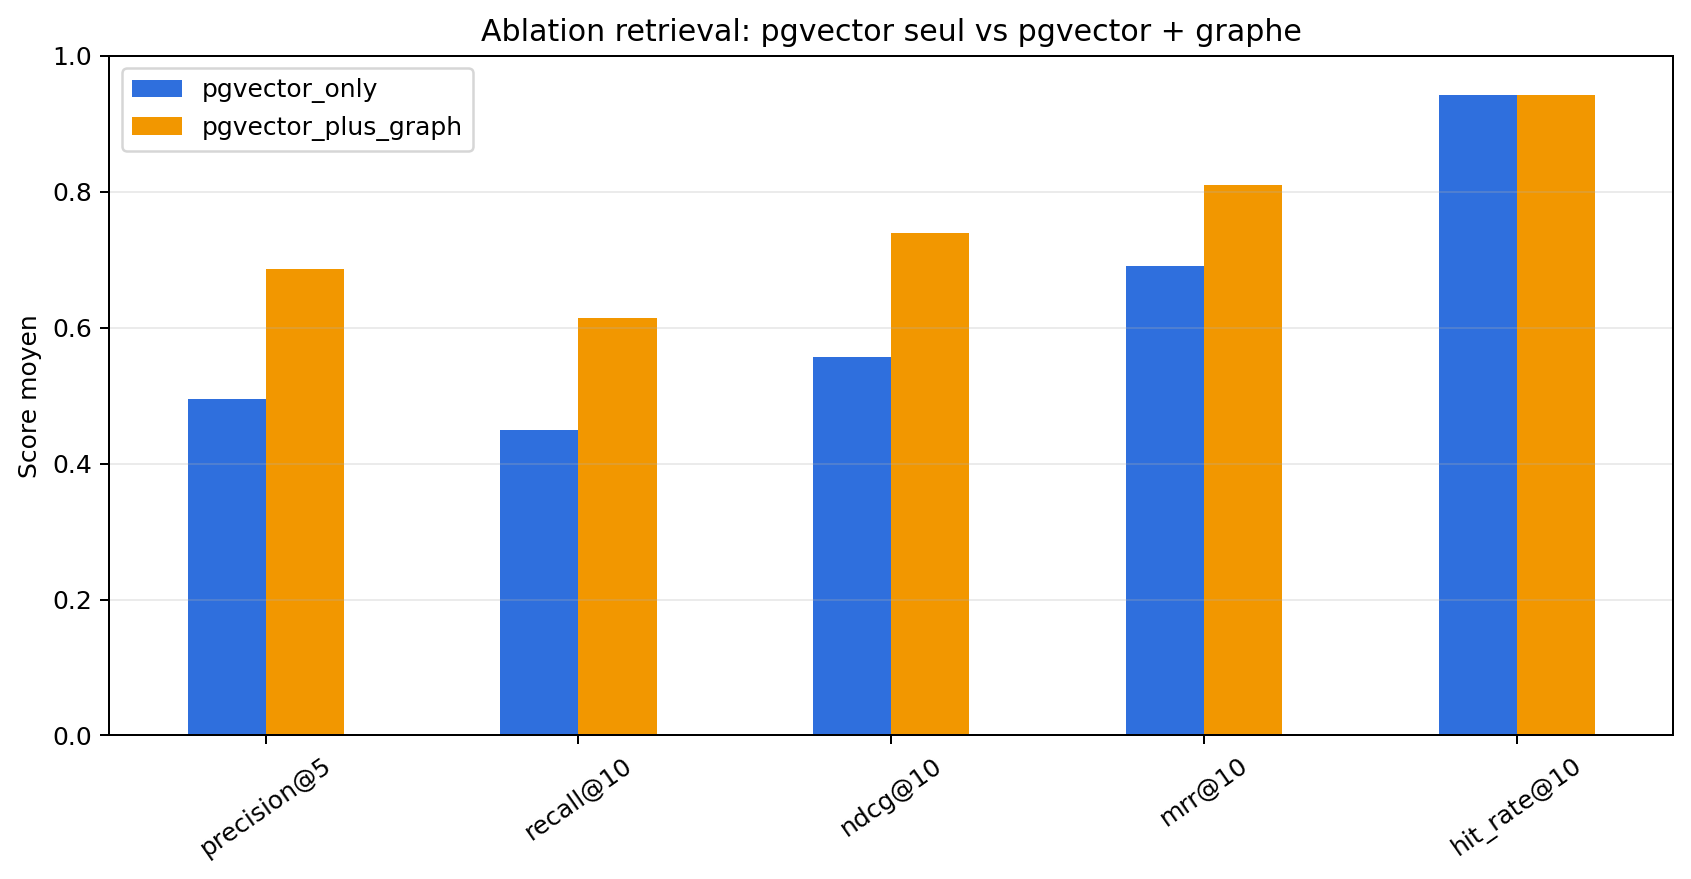
\includegraphics[width=\linewidth,height=5.15cm,keepaspectratio]{figures/generated/evaluation/ablation_metrics_comparison.png}
    \column{0.35\textwidth}
      \begin{block}{Ablation contrôlée}
        69 candidats, même pool initial de 30 offres.
      \end{block}
      \scriptsize
      \begin{tabular}{lcc}
        \toprule
        & pgvector & + graphe\\
        \midrule
        NDCG@10 & 0,5575 & \textbf{0,7392}\\
        MRR@10 & 0,6908 & \textbf{0,8093}\\
        Recall@10 & 0,4491 & \textbf{0,6147}\\
        \bottomrule
      \end{tabular}

      \vspace{0.22cm}
      \alert{C'est le résultat le mieux identifié du mémoire}, mais la pertinence
      reste définie par un proxy.
  \end{columns}
  \sourceNote{Sortie \texttt{13\_ablation\_pgvector\_neo4j\_reranking.csv} ; 11 candidats initialement tirés exclus après erreurs techniques.}
\end{frame}

\begin{frame}{Preuve 3 — expliquer, puis contrôler l'ancrage}
  \begin{columns}[T,onlytextwidth]
    \column{0.48\textwidth}
      \begin{block}{Explication relationnelle}
        Pour chaque candidat--offre :
        \begin{itemize}
          \item compétences possédées et requises ;
          \item couverture $|K_c\cap K_o|/|K_o|$ ;
          \item compétences manquantes $K_o\setminus K_c$ ;
          \item chemins métier--formation mobilisés.
        \end{itemize}
      \end{block}
    \column{0.48\textwidth}
      \begin{block}{Critic contrastif}
        Au seuil 0,46, le protocole accepte 50/51 vrais contextes et rejette
        51/51 contextes mélangés.

        \vspace{0.20cm}
        \alert{Il mesure un ancrage lexical, pas la vérité métier.}
      \end{block}
  \end{columns}
  \vspace{0.23cm}
  \begin{center}
    \pill{KmerGreen}{APPORT}\quad Une recommandation devient inspectable.\qquad
    \pill{KmerRed}{LIMITE}\quad L'explication n'est pas encore validée par l'utilisateur.
  \end{center}
  \sourceNote{Mémoire, chapitres d'évaluation et de discussion ; évaluation RAG \citep{es2024ragas}.}
\end{frame}

\begin{frame}{Ce que les résultats autorisent — et interdisent}
  \begin{columns}[T,onlytextwidth]
    \column{0.48\textwidth}
      \begin{block}{\centering Conclusions défendables}
        \begin{itemize}
          \item faisabilité d'un pipeline modulaire ;
          \item gain interne du graphe sur le même vivier ;
          \item production d'un \textit{skill gap} traçable ;
          \item mécanisme expérimental de contrôle des réponses.
        \end{itemize}
      \end{block}
    \column{0.48\textwidth}
      \begin{alertblock}{\centering Conclusions non établies}
        \begin{itemize}
          \item meilleure qualité réelle des recrutements ;
          \item amélioration causale de l'emploi ;
          \item absence de biais entre sous-groupes ;
          \item robustesse temporelle et intersectorielle ;
          \item utilité des explications pour les décideurs.
        \end{itemize}
      \end{alertblock}
  \end{columns}
  \vspace{-0.06cm}
  \begin{center}
    \textbf{La thèse ne prolongera pas une promesse : elle organisera des tests
    capables de la réfuter.}
  \end{center}
  \sourceNote{Discussion et limites du mémoire et de l'article scientifique.}
\end{frame}

\section{Programme doctoral}

\begin{frame}{Question doctorale proposée}
  \vspace{0.20cm}
  \begin{center}
    \begin{tikzpicture}
      \node[rounded corners=4pt,draw=KmerNavy,very thick,fill=KmerNavy!5,
        text width=12.4cm,align=center,inner sep=12pt]
      {\Large\bfseries\color{KmerNavy}
      Comment concevoir et évaluer des systèmes hybrides emploi--compétences
      qui demeurent pertinents, explicables et équitables sous hétérogénéité des
      données, changement de domaine et contrôle humain ?};
    \end{tikzpicture}
  \end{center}
  \vspace{0.36cm}
  \begin{columns}[T,onlytextwidth]
    \column{0.31\textwidth}\centering
      \pill{KmerBlue}{PERTINENCE}\par\smallskip
      annotations expertes et évaluation hors échantillon
    \column{0.31\textwidth}\centering
      \pill{KmerGreen}{ROBUSTESSE}\par\smallskip
      secteurs, temps, sources et sous-groupes
    \column{0.31\textwidth}\centering
      \pill{KmerMagenta}{DÉCISION HUMAINE}\par\smallskip
      compréhension, calibration et contestabilité
  \end{columns}
  \sourceNote{Proposition originale dérivée des limites empiriques du mémoire.}
\end{frame}

\begin{frame}{Quatre questions de recherche, une progression logique}
  \begin{enumerate}
    \item[\textcolor{KmerBlue}{\bfseries RQ1}] \textbf{Validité.} Comment construire
      une vérité terrain indépendante et mesurer l'accord entre experts ?
    \item[\textcolor{KmerGreen}{\bfseries RQ2}] \textbf{Généralisation.} Quels
      composants restent performants sous changement temporel, sectoriel ou lexical ?
    \item[\textcolor{KmerPurple}{\bfseries RQ3}] \textbf{Confiance.} Les chemins du
      graphe et les preuves récupérées améliorent-ils réellement la compréhension et
      la calibration du jugement humain ?
    \item[\textcolor{KmerMagenta}{\bfseries RQ4}] \textbf{Équité.} Où apparaissent
      les écarts de performance entre sous-groupes, et quelles contraintes réduisent
      les erreurs injustifiées sans masquer les compromis ?
  \end{enumerate}
  \vspace{0.30cm}
  \begin{center}
    \textbf{Unité d'analyse :} la recommandation candidat--offre, son rang, ses
    preuves, son incertitude et son effet sur un évaluateur humain.
  \end{center}
\end{frame}

\begin{frame}{Hypothèses falsifiables — pas de promesse technologique}
  \scriptsize
  \renewcommand{\arraystretch}{1.04}
  \begin{tabularx}{\textwidth}{>{\bfseries\color{KmerNavy}}p{0.65cm}X>{\raggedright\arraybackslash}p{3.8cm}}
    \toprule
    & Hypothèse & Test décisif\\
    \midrule
    H1 & L'adaptation au domaine améliore le classement jugé pertinent par des experts indépendants. & Holdout temporel ; comparaison BM25, encodeurs génériques et adapté.\\
    H2 & Le reranking relationnel apporte un gain au-delà du retrieval sémantique. & Ablations à pool constant ; intervalles bootstrap ; tests appariés.\\
    H3 & Une explication fondée sur des preuves améliore la décision humaine. & Expérience contrôlée : liste seule vs score vs explication + incertitude.\\
    H4 & Des contraintes explicites peuvent réduire certains écarts d'erreur entre sous-groupes. & Audit désagrégé ; seuils et compromis performance--équité préspécifiés.\\
    \bottomrule
  \end{tabularx}
  \sourceNote{Les hypothèses finales seront resserrées avec le directeur de thèse et préenregistrées avant l'évaluation confirmatoire.}
\end{frame}

\begin{frame}{Design empirique : construction, calibration, preuve}
  \begin{center}
  \begin{tikzpicture}[node distance=0.34cm,every node/.style={font=\scriptsize}]
    \tikzset{stage/.style={rounded corners,draw=KmerNavy,very thick,fill=KmerGray,
      text width=2.10cm,minimum height=1.05cm,align=center,inner xsep=2pt}}
    \node[stage] (a) {\textbf{1. Données}\\versionnées, dédupliquées,\\audit de couverture};
    \node[stage,right=of a] (b) {\textbf{2. Annotation}\\plusieurs experts,\\accord et désaccord};
    \node[stage,right=of b] (c) {\textbf{3. Modélisation}\\baselines, ablations,\\calibration séparée};
    \node[stage,right=of c] (d) {\textbf{4. Évaluation}\\holdout temporel,\\incertitude, sous-groupes};
    \node[stage,right=of d] (e) {\textbf{5. Utilisateurs}\\expérience contrôlée,\\qualitatif + quantitatif};
    \foreach \x/\y in {a/b,b/c,c/d,d/e}{\draw[-{Stealth},thick,KmerMagenta] (\x) -- (\y);}
  \end{tikzpicture}
  \end{center}
  \vspace{0.30cm}
  \begin{columns}[T,onlytextwidth]
    \column{0.48\textwidth}
      \begin{block}{Mesures système}
        NDCG/MRR/Recall, calibration, robustesse, latence, coût et fidélité aux preuves.
      \end{block}
    \column{0.48\textwidth}
      \begin{block}{Mesures humaines}
        précision de décision, temps, confiance calibrée, compréhension et capacité de contestation.
      \end{block}
  \end{columns}
\end{frame}

\begin{frame}{Rigueur statistique et garde-fous méthodologiques}
  \small
  \begin{columns}[T,onlytextwidth]
    \column{0.48\textwidth}
      \begin{block}{Inférence}
        \begin{itemize}
          \item tailles d'effet et intervalles de confiance ;
          \item bootstrap par requête/candidat ;
          \item tests appariés et correction de multiplicité ;
          \item analyse de puissance pour l'étude utilisateur ;
          \item sensibilité aux définitions de pertinence.
        \end{itemize}
      \end{block}
    \column{0.48\textwidth}
      \begin{block}{Prévention des faux progrès}
        \begin{itemize}
          \item jeu de test gelé et holdout temporel ;
          \item proxy interdit comme vérité finale ;
          \item ablations à vivier identique ;
          \item données manquantes et échecs explicités ;
          \item protocole, code et versions archivés.
        \end{itemize}
      \end{block}
  \end{columns}
  \vspace{0.04cm}
  \begin{center}\scriptsize
    \pill{KmerRed}{LIGNE ROUGE}\quad
    Pas d'impact sur l'emploi revendiqué sans design causal approprié.
  \end{center}
\end{frame}

\begin{frame}{Feuille de route doctorale sur 36 mois}
  \begin{center}
  \begin{tikzpicture}[x=0.31cm,y=1cm,every node/.style={font=\scriptsize}]
    \draw[->,very thick,KmerNavy] (0,0) -- (36.8,0);
    \foreach \x/\lab in {0/M0,6/M6,14/M14,22/M22,29/M29,36/M36}{
      \draw[KmerNavy] (\x,-0.08)--(\x,0.08) node[below=2pt]{\lab};}
    \fill[KmerBlue!75] (0,0.28) rectangle (6,0.82);
    \node[white,align=center] at (3,0.55) {\bfseries WP1};
    \fill[KmerGreen!80] (6,0.28) rectangle (14,0.82);
    \node[white,align=center] at (10,0.55) {\bfseries WP2};
    \fill[KmerPurple!80] (14,0.28) rectangle (22,0.82);
    \node[white,align=center] at (18,0.55) {\bfseries WP3};
    \fill[KmerMagenta!80] (22,0.28) rectangle (29,0.82);
    \node[white,align=center] at (25.5,0.55) {\bfseries WP4};
    \fill[KmerGold!90!black] (29,0.28) rectangle (36,0.82);
    \node[white,align=center] at (32.5,0.55) {\bfseries WP5};
  \end{tikzpicture}
  \end{center}
  \vspace{0.35cm}
  \begin{columns}[T,onlytextwidth]
    \column{0.31\textwidth}
      \textbf{Année 1}\par
      Gouvernance des données, revue systématique, annotation experte, baselines.
    \column{0.31\textwidth}
      \textbf{Année 2}\par
      Nouveaux modèles hybrides, robustesse, incertitude et audit par sous-groupes.
    \column{0.31\textwidth}
      \textbf{Année 3}\par
      Étude utilisateur, pilote encadré, articles, synthèse et transfert reproductible.
  \end{columns}
  \vspace{0.24cm}
  \begin{center}\small
    Jalons : \pill{KmerBlue}{J1 benchmark} \quad
    \pill{KmerPurple}{J2 modèle robuste} \quad
    \pill{KmerMagenta}{J3 preuve utilisateur} \quad
    \pill{KmerGold}{J4 thèse}
  \end{center}
\end{frame}

\begin{frame}{Contributions scientifiques attendues}
  \begin{columns}[T,onlytextwidth]
    \column{0.31\textwidth}
      \begin{block}{Article 1}
        \textbf{Benchmark emploi--compétences}\par
        Annotation multi-experts, temporalité, désaccord et protocole de référence.
      \end{block}
    \column{0.31\textwidth}
      \begin{block}{Article 2}
        \textbf{Retrieval hybride robuste}\par
        Ablations, incertitude, changement de domaine et contraintes relationnelles.
      \end{block}
    \column{0.31\textwidth}
      \begin{block}{Article 3}
        \textbf{Explications utiles}\par
        Effet des preuves et du \textit{skill gap} sur la qualité de décision humaine.
      \end{block}
  \end{columns}
  \vspace{0.28cm}
  \begin{center}
    \begin{tikzpicture}
      \node[rounded corners,fill=KmerNavy,text=white,text width=12.2cm,
        align=center,inner sep=9pt]
      {\bfseries Livrable transversal : un cadre reproductible et auditable,
       transférable à d'autres marchés où les historiques d'interaction sont rares.};
    \end{tikzpicture}
  \end{center}
  \sourceNote{Les cibles de publication et le périmètre exact seront définis avec l'équipe d'accueil.}
\end{frame}

\begin{frame}{Risques anticipés — et décisions prévues}
  \scriptsize
  \renewcommand{\arraystretch}{1.03}
  \begin{tabularx}{\textwidth}{>{\raggedright\arraybackslash\bfseries\color{KmerRed}}p{3.0cm}X>{\raggedright\arraybackslash}p{4.0cm}}
    \toprule
    Risque & Conséquence & Réponse méthodologique\\
    \midrule
    Peu d'annotations expertes & vérité terrain fragile & échantillonnage actif, double codage, analyse du désaccord\\
    Données privées/incomplètes & reproductibilité limitée & artefacts anonymisés, contrats de données, jeux synthétiques de test\\
    Dérive temporelle/sectorielle & performance non transportable & splits temporels, stress tests, recalibration documentée\\
    Biais de sélection & écarts invisibles & audits désagrégés, fiches de données, limites d'usage explicites\\
    Explication persuasive mais fausse & confiance mal placée & citations de preuves, critic séparé, possibilité d'abstention et recours humain\\
    \bottomrule
  \end{tabularx}
\end{frame}

\section{Partenariat scientifique}

\begin{frame}{Ce que j'apporte — ce que je recherche}
  \small
  \begin{columns}[T,onlytextwidth]
    \column{0.48\textwidth}
      \begin{block}{Actifs immédiatement mobilisables}
        \begin{itemize}
          \item une double formation statistique, économique et Data Science
          \item un pipeline complet déjà implémenté
          \item un corpus pilote et des référentiels structurés
          \item une évaluation reproductible et une connaissance du contexte camerounais.
        \end{itemize}
      \end{block}
    \column{0.48\textwidth}
      \begin{block}{Encadrement recherché}
        \begin{itemize}
          \item resserrer la question et l'ancrage théorique
          \item challenger le design expérimental et statistique
          \item accéder à un environnement exigeant et à des partenaires d'annotation
          \item viser des contributions publiables, pas une simple plateforme.
        \end{itemize}
      \end{block}
  \end{columns}
  \vspace{0.02cm}
  \begin{center}\scriptsize
    \pill{KmerMagenta}{POSTURE}\quad
    Je cherche un encadrement qui teste mes idées, pas une validation du prototype.
  \end{center}
\end{frame}

\begin{frame}{Espace de co-construction avec le directeur de thèse}
  \begin{columns}[T,onlytextwidth]
    \column{0.31\textwidth}
      \begin{block}{À fixer ensemble}
        question centrale, terrain, population, accès aux experts, discipline
        d'inscription et contraintes éthiques.
      \end{block}
    \column{0.31\textwidth}
      \begin{block}{À challenger}
        définition de pertinence, hypothèses, identification, comparateurs,
        métriques et stratégie de publication.
      \end{block}
    \column{0.31\textwidth}
      \begin{block}{À préserver}
        séparation système/métier, traçabilité, décision humaine et honnêteté sur
        l'incertitude.
      \end{block}
  \end{columns}
  \vspace{0.35cm}
  \begin{center}
    \Large\bfseries\color{KmerNavy}
    Mon objectif : passer d'un système qui fonctionne\par
    à une connaissance qui résiste à la critique.
  \end{center}
\end{frame}

\begin{frame}{Proposition de collaboration doctorale}
  \vspace{0.08cm}
  \begin{center}
    {\Large\bfseries\color{KmerNavy}
      Un terrain pertinent. Un prototype exécutable.\par
      Des limites explicites. Des hypothèses falsifiables.}

    \vspace{0.25cm}
    \begin{tikzpicture}
      \node[rounded corners=5pt,fill=KmerNavy,text=white,text width=12.0cm,
        align=center,inner sep=10pt]
      {\Large\bfseries
      Je vous propose de transformer ce point de départ en un programme doctoral
      rigoureux sur la recommandation hybride, l'explicabilité et la décision humaine.};
    \end{tikzpicture}

    \vspace{0.25cm}
    \pill{KmerMagenta}{PROCHAINE ÉTAPE}\quad
    Discuter l'alignement avec vos axes, le terrain d'évaluation et un premier
    protocole d'annotation.

    \vspace{0.22cm}
    {\large\bfseries Merci pour votre attention — discussion}
  \end{center}
\end{frame}

% -----------------------------------------------------------------------------
% ANNEXES TECHNIQUES — mobilisables uniquement si le professeur approfondit.
% -----------------------------------------------------------------------------
\appendix

\begin{frame}{Annexe — équations du moteur hybride}
  \begin{align*}
    s_{\mathrm{vec}}(q,o)
      &= \frac{e(q)\cdot e(o)}{\lVert e(q)\rVert_2\lVert e(o)\rVert_2},\\[0.25cm]
    s_{\mathrm{graph}}(c,o)
      &= \frac{|K_c\cap K_o|}{|K_o|},\\[0.25cm]
    s_{\mathrm{hyb}}(c,o)
      &= \alpha s_{\mathrm{vec}}(c,o)+\beta s_{\mathrm{graph}}(c,o),
      \qquad \alpha+\beta=1,\\[0.25cm]
    \mathrm{gap}(c,o)
      &= K_o\setminus K_c.
  \end{align*}
  \begin{center}
    \small La calibration dépend de la fonction objectif et du proxy : elle n'est
    pas transportable sans réestimation.
  \end{center}
\end{frame}

\begin{frame}{Annexe — protocole d'évaluation actuel}
  \small
  \begin{tabularx}{\textwidth}{>{\bfseries}p{3.2cm}p{3.4cm}X}
    \toprule
    Brique & Échantillon & Portée\\
    \midrule
    Encodeur adapté & 953 paires de test & self-retrieval sur paires offre--description\\
    Ablation du graphe & 69 candidats, pool de 30 offres & comparaison à vivier constant selon proxy\\
    Optuna & 690 couples, 500 essais & poids dépendants de l'objectif et de l'échantillon\\
    Critic & 51 vrais + 51 contextes mélangés & ancrage lexical contrastif au seuil 0,46\\
    \bottomrule
  \end{tabularx}
  \vspace{0.38cm}
  \begin{alertblock}{Limite commune}
    Aucune de ces évaluations ne remplace une annotation métier indépendante ou
    une étude utilisateur confirmatoire.
  \end{alertblock}
\end{frame}

\begin{frame}[allowframebreaks]{Références essentielles}
  \footnotesize
  \bibliographystyle{plainnat}
  \bibliography{references}
\end{frame}

\end{document}
